\documentclass{book}
\usepackage[spanish]{babel}
\usepackage[utf8]{inputenc}
\usepackage[colorlinks = true, linkcolor = magenta]{hyperref}
\usepackage{graphicx}

\begin{document}

	\begin{titlepage}
		\centering
		{\bfseries\LARGE Universidad de La Habana \par }
		\vspace{1cm}
		{\scshape\LARGE Facultad de Matem\'atica y Computaci\'on \par}
		\vspace{3cm}
		{\scshape\Huge Aprendizaje Profundo en la clasificaci\'on de Im\'agenes  \par}
		\vspace{3cm}
		{\itshape\Large Proyecto Final de Inteligencia Artificial \par}
		\vfill
		{\Large \underline{Integrantes:} \par}
		{\Large Sheyla Cruz Castro C-512 \par}
		{\Large Laura Brito Guerrero C-512 \par}
		{\Large Ariel Antonio Huerta Mart\'in C-512 \par}
		\vfill
	\end{titlepage}
	
	\tableofcontents
	\chapter{Introducci\'on}
		\section{Presentaci\'on del objetivo} \label{1p}
			\begin{center}
				\textit{Deep Learning in images classification (Aprendizaje Profundo en la clasificaci\'on de im\'agenes)}
			\end{center}
				

			Se tiene un dataset de im\'agenes tomadas por microscopios de barrido, cada conjunto de im\'agenes se encuentra clasificada. El objetivo principal dada una imagen arbitraria, es identificar si pertenece a alguna clasificaci\'on del dataset que se tiene. A grandes rasgos, se pretende realizar la clasificaci\'on de im\'agenes mediante el aprendizaje profundo. La optimalidad de los casos correctos de la aplicaci\'on va a ser directamente proporcional con el tiempo asignado al proyecto. Para generar estos fines, se va a llevar a cabo la implementaci\'on en python, con el auxilio de la biblioteca TensorFlow.
			Con respecto a la relaci\'on que tiene este trabajo con otras asignaturas se puede decir que es bastante amplia. Vamos a emplear conocimiento de procesamiento de im\'agenes, tales como la convoluci\'on, funciones activadoras (en este caso: ReLu), y la t\'ecnica maxpolling para disminuir el tama\~no de la imagen y as\'i mantener una eficiencia espacial. Por otra parte, el aprendizaje profundo consta de una estructura de datos basada en grafos, donde en una parte espec\'ifica tendremos como bien conocida es: \textit{Fully Connected Layers}, que no es m\'as que un grafo bipartito completo el cual interviene en el proceso de la clasificaci\'on. Y siendo m\'as espec\'ifico en la parte de la clasificaci\'on, se utilizar\'an modelos probabilistas. Por lo tanto, a modo de resumen tenemos que su relaci\'on con otras asignaturas es perenne, algunas de estas son : Procesamiento de Im\'agenes, Probabilidades, Estructura de datos y algoritmos.

			
		\section{Estructura} \label{estructSec}
			En la carpeta \textbf{src} se encuentra la implementaci\'on del proyecto. Dentro se encuentran los ficheros \textbf{train.py}, el cual es el primero que se tiene que ejecutar pues el mismo se encarga de entrenar el modelo, proceso en el cual la m\'aquina aprende de las im\'agenes de entrenamiento y eval\'ua la precisi\'on con respecto a las im\'agenes de validaci\'on; y el otro fichero es \textbf{predict.py} el cual resuelve la problem\'atica de la clasificaci\'on leyendo el modelo anteriormente entrenado dada una imagen de entrada arbitraria. \\
			Se encuentra la carpeta \textbf{dataset}, en la cual se encuentran los conjuntos de im\'agenes de entrenamiento y de validaci\'on respectivamente. En este proyecto se va a clasificar en tres clases: \textit{Plasmodium Falciparum(Malaria)}; \textit{Sars-Cov2(Covid-19)}; y \textit{Vibrio Cholerae(C\'olera)}. Esto conlleva que exista una carpeta con im\'agenes de cada clase en cada conjunto.
	
	\chapter{Introducci\'on a las redes neuronales profundas}
		\section{Un poco de teor\'ia ...}
			\textit{Deep Convolutional Neural Networks (Redes neuronales convolucionales profundas)} 
			La historia de las CNN profundas se remonta a principios de la d\'ecada de 1980, pero solo hasta la d\'ecada de 2010, los investigadores lograron una alta precisi\'on en la resoluci\'on de tareas de reconocimiento de im\'agenes con redes neuronales convolucionales profundas. La manera en que lo lograron fue comenzando a entrenar e implementar CNN utilizando unidades de procesamiento gr\'aficos (GPU) que aceleran significativamente los sistemas complejos basados en redes neuronales. La cantidad de datos de entrenamiento (fotos o videos) tambi\'en aument\'o porque las c\'amaras de los tel\'efonos m\'ovil y las c\'amaras digitales comenzaron a desarrollarse r\'apidamente y se volvieron asequibles. \\
			
			Actualmente es com\'unmente utilizado para el reconocimiento de las im\'agenes en la instancia de pesos fijados con el algoritmo de \textit{back propagation network}. Ayuda a resolver los problemas de an\'alisis de datos de alta dimensi\'on en espacio el cual provee una clase de algoritmos y desbloquea la compleja situaci\'on gracias a su propiedad sim\'etrica. \\
			El aprendizaje profundo en la clasificaci\'on de im\'agenes basada en redes neuronales inicia la nueva revoluci\'on en la inteligencia artificial y es relevante en distintos dominios: en el an\'alisis de la se\~nal de audio y video, reconocimiento facial, reconocimiento de desastres, reconocimiento de voz, visi\'on de computadora y en el procesamiento del lenguaje automatizado. \\
			Es un conjunto de algoritmos donde prepara a un modelo con gran nivel de abstracci\'on en datos por el uso de un grafo profundo con el procesamiento de m\'ultiples	capas. Ha ganado gran popularidad en la \'ultima d\'ecada por su habilidad de aprender representaci\'on de datos en una manera supervisada o no supervisada y generaliza los conjuntos de datos con el uso de representaciones jer\'arquicas. \\
			La esencial propiedad de sus algoritmos es la extracci\'on autom\'atica de rasgos. Esto significa que el algoritmo autom\'aticamente comprende los rasgos relevantes requeridos para la soluci\'on del problema. Las CNN tiene tres capas invisibles principales, usualmente varias capas y como son profundas tienen m\'as de un estado de no linealidad en las transformaciones. Cada capa invisible se compone de un conjunto de neuronas responsables de entrenar un \'unico conjunto de rasgos basados en la salida de la capa anterior. Como el n\'umero de las capas crece, la complejidad y abstracci\'on de los datos tambi\'en crece.
		\section{Convolution}
			La convoluci\'on es una transformaci\'on matem\'atica de dos funciones que genera una tercera funci\'on. Su representaci\'on matem\'atica es la siguiente:
			\begin{equation}
				(uv)(x)= \int u(x - t)v(t)dt
			\end{equation}
			Gr\'aficamente se visualiza en la siguiente imagen:
			\begin{center}
				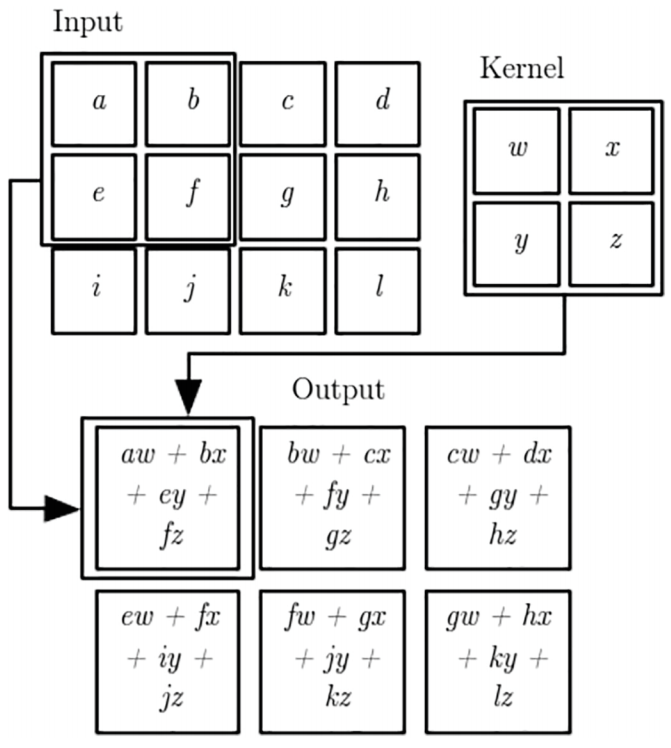
\includegraphics[width=8cm]{15.png}
			\end{center}
			En inteligencia artificial, las redes convoluciones profundas se aplica a m\'ultiples cascadas de kernels de convoluci\'on con aplicaciones de aprendizaje profundo.
			\subsection{Convolution Layer}
				Esta es la primera de las capas, una de las m\'as importantes y tiene gran aplicaci\'on en el reconocimiento de im\'agenes. Tiene tres par\'ametros fundamentales: \textit{depth}(la profundidad del volumen de salida controla el n\'umero de neuronas que conecta con la capa en la misma regi\'on del volumen de entrada), \textit{stride}(controla como las columnas profundas alrededor de las dimensiones espaciales(ancho y altura) son localizadas, si el stride es 1 entonces el se mueve los filtros un pixel por tiempo) y \textit{zero-padding}(coloca zeros en los bordes de la imagen de entrada, en ocasiones no se desea variar las dimensiones de la imagen de entrada).
		\section{ReLu}
			\textbf{ReLu}: Rectified Linear Units, es una funci\'on de activaci\'on que se define:
			\begin{equation}
				f(x) = max(0,x)
			\end{equation}
			Su objetivo principal es quitar informaci\'on innecesaria brindada por la imagen luego de una tranformaci\'on por convoluci\'on (en este caso).
			\subsection{ReLu Layer}
				Es la capa de neuronas que se encarga de funciones de no saturaci\'on y no linealidad o de la funci\'on loss. Sus resultados en la red neuronal explican rapidez y claridad en la etapa de entrenamiento, puesto que limpia todos aquellos p\'ixeles que no contengan informaci\'on necesaria para el aprendizaje.
		\section{Max Polling}
			Se encarga de reducir o simplificar la dimensi\'on espacial de la informaci\'on capturada en la imagen. 
			\begin{center}
				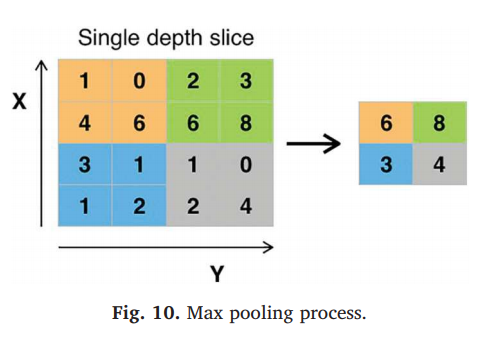
\includegraphics[width=6cm]{16.png}
			\end{center}
			\subsection{Polling Layer}
				La m\'as utilizada es \textbf{max polling}, ya que est\'a caracterizada por ser r\'apida en convergencia.Como se explica en la imagen anterior se toma un tama\~no de kernel y se recorre el volumen de entrada escogiendo cada vez el valor mayor en cada ventana apreciada por el tama\~no del kernel.
		\section{Fully Connected Layer}
			La entrada de esta capa es un vector de n\'umeros. Cada entrada es conectada a cada una de las salidas conocido por el t\'ermino \textbf{Fully Connected}. Contiene acerca del 90 porciento de los par\'ametros de la red. Esta capa toma b\'asicamente como entrada la salida de la \'ultima capa de \textbf{Polling} y su salida es un vector \textbf{N-dimensional}, donde \textbf{N} es el n\'umero de clases a clasificar.
		\section{Loss Layer}
			Toma la salida del modelo y el \textit{target} y computa su valor que no es m\'as que la distancia entre ambas entradas. Para su c\'alculo tiene dos funciones principales:
			\begin{enumerate}
			\item Forward pass: calcular el valor de loss basado en la entrada y el valor del \textit{target},
			\item Backward pass: calcular el gradiente de la funci\'on loss asociado con el criterio y retorna el valor.
			\end{enumerate}
			A estas funciones se le hacen menci\'on a continuaci\'on.
		\section{Back propagation Algorithm}
			El algoritmo de \textbf{back \ propagation} se introdujo originalmente en la d\'ecada de 1970, pero su importancia no se apreci\'o completamente hasta un famoso art\'iculo de 1986 de David Rumelhart, Geoffrey Hinton y Ronald Williams. La retropropagaci\'on funciona mucho m\'as r\'apido que los enfoques de aprendizaje anteriores, lo que hace posible utilizar redes neuronales para resolver problemas que anteriormente hab\'ian sido insolubles. \\
			Se dice que la transformaci\'on implementada por una capa es parametrizada por \textit{pesos (weights)}, inicialmente estas variables tienen valores aleatorios y es el algoritmo de \textit{back propagation} el que ajusta estos \textit{pesos}. Una red neuronal profunda puede tener diez millones de par\'ametros, buscar el valor correcto para todos ellos es una tarea exhaustiva y m\'as que al cambiar un solo valor de ellos todos los dem\'as se deben actualizar, ya que afecta sus comportamientos. \\
			Para controlar la salida de una red neuronal se necesita habilitar una medida que nos diga que tan r\'apido est\'a aprendiendo para llegar a la salida que se espera, este es el trabajo de la \textit{function loss}, a veces tambi\'en llamada \textit{funci\'on objetiva} o \textit{funci\'on de costo}. La funci\'on de p\'erdida toma las predicciones de la red y los verdaderos targets y computa la distancia que existe entre ellos capturando como la red termina en un ejemplo espec\'ifico. \\
			La funci\'on del optimizador es implementar la llamada del algoritmo \textit{Back Propagation}: el algoritmo central del aprendizaje profundo. Como bien se comenta anteriormente los pesos son asignados aleatoriamente donde la red implementa una serie de transformaciones aleatorias, cuando los pesos se ajustan un poco en la direcci\'on correcta, el valor de la funci\'on de p\'erdida decrece, lo que se quiere lograr es tener el menor valor de p\'erdida posible en el ajuste de los pesos. \\
			\begin{center}
				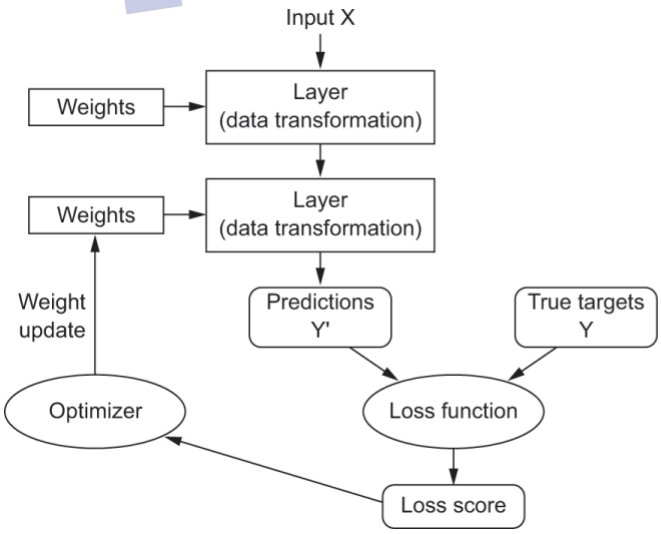
\includegraphics[width=5cm]{4.png}
			\end{center}

			Ahora bien, en el ajuste de los pesos interfieren dos sentidos en el \textit{back propagation}: \textit{forward pass} y \textit{backward pass}. Como \textit{loss\underline{ }val} es la diferencia entre el valor de predicci\'on y el valor de \textit{true target}. Se definen los pasos en la siguiente figura, la primera se refiere a \textit{forward pass} y la segunda a \textit{backward pass}: \\
				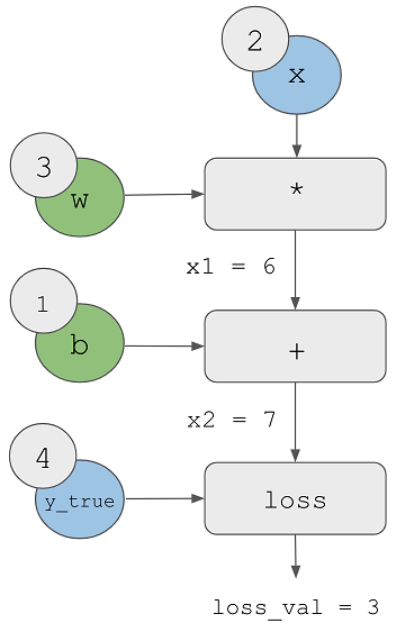
\includegraphics[width=5cm]{12.png}
				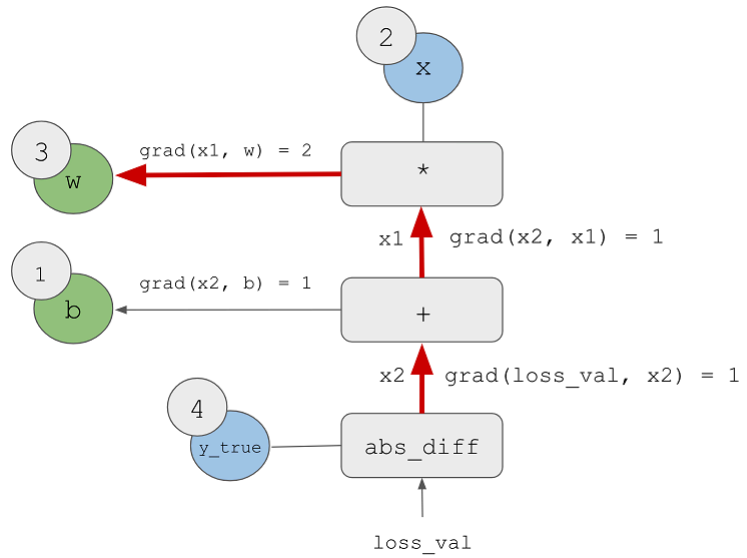
\includegraphics[width=9cm, height=8cm]{14.png}
			Tener en cuenta que las operaciones que se le realiza por capa viene dada por la funci\'on activadora \textbf{ReLu}, ya que ocurre una multiplicaci\'on(operaci\'on de convoluci\'on) y una suma con un \textit{sesgo}, valor que se aprecia en \textit{b}, hablando espec\'ificamente en el \textit{forward pass}. Con respecto a \textit{backward pass} se deben tener en cuenta una serie de consideraciones ya que \textit{grad(a,b)} no es igual a \textit{grad(b,a)}, ya que estamos hablando de aristas invertidas en el grafo. Explicando el \textit{backward pass} tenemos:
			\begin{enumerate}
				\item \textit{grad(loss\underline{ }val, x2)=1} ya que como \textit{x2} var\'ia por un monto \textit{epsilon}, \\		\textit{loss\underline{ }val=abs(4-x2)} var\'ia en el mismo monto.
				\item \textit{grad(x2,x1)=1} como \textit{x1} var\'ia por un monto epsilon igual, \textit{x2=x1+b=x1+1} var\'ia en el mismo monto.
				\item \textit{grad(x2,b)=1} como \textit{b} var\'ia por un monto epsilon, \textit{x2=x1+b=6+b} var\'ia en el mismo monto.
				\item \textit{grad(x1,w)=2} como \textit{w} var\'ia por un monto epsilon, \textit{x1=x*w=2*w} var\'ia por \textit{2 * epsilon}.
			\end{enumerate}
		\section{Proceso de entrenamiento}
			Un sistema debe aprender primero sus caracter\'isticas. Debe entrenarse para predecir si un objeto es \textbf{X}, \textbf{Y}, …. Los modelos de aprendizaje profundo aprenden estas caracter\'isticas de una manera diferente a los modelos de aprendizaje tradicional. Es por eso que los enfoques de entrenamiento de modelos tambi\'en son diferentes. \\
			Para construir un modelo ML que pueda, los cient\'ificos de datos deben especificar qu\'e caracter\'isticas de entrada \textit{(Propiedades del problema)} considerara el modelo al predecir un resultado. Eso puede ser el tama\~no del virus, su fisonom\'ia, el contorno, sus interacciones. El proceso de construcci\'on de funciones utilizando el conocimiento del dominio se denomina \textit{ingenier\'ia de funciones}. \\
			Para entrenar un modelo se deben reunir las caracter\'isticas de miles de millones de datos de los virus que se quieren clasificar. No se pueden construir funciones precisas que funcionen para cada imagen posible teniendo en cuenta complicaciones tales como la variabilidad del objeto dependiente del punto de vista, el desorden del fondo, las condiciones de iluminaci\'on o la deformaci\'on de la imagen. Deber\'ia haber otro enfoque, y existe gracias a la naturaleza de las redes neuronales. \\
			Las redes neuronales aprenden funciones directamente de los datos con los que se entrenan, por lo que los especialistas no necesitan extraer funciones manualmente. \\
			\textit{El poder de las redes neuronales proviene de su capacidad para aprender la representaci\'on en sus datos de entrenamiento y como relacionarlos mejor con la variable de salida que desea predecir. En este sentido, las redes neuronales aprenden a mapear. Matem\'aticamente, son capaces de aprender cualquier funci\'on de mapeo y se ha demostrado que son algoritmos de aproximaci\'on universales}, se\~nala Jason Brownlee en Crash Course on Multi-layer Perceptron Neural Networks. \\
			Los datos de entrenamiento, en este caso, son un gran conjunto de datos que contiene muchos ejemplos de cada clase de imagen. Ej.: el conjunto de im\'agenes de \textbf{ImageNet} contiene m\'as de 14 millones de im\'agenes anotadas por humanos que representan 21841 conceptos (cjtos de sin\'onimos o conjuntos de sincronizaci\'on seg\'un la jerarqu\'ia de \textbf{WordNet}), con un promedio de 1000 im\'agenes por concepto. \\
			Cada imagen se encuentra anotada (etiquetada) con una categor\'ia a la que pertenece: conjunto de virus. El algoritmo explora estos ejemplos, aprende sobre las caracter\'isticas visuales de cada categor\'ia y finalmente aprende a reconocer cada clase de imagen. El estilo de entrenamiento modelo se llama: \textit{APRENDIZAJE SUPERVISADO}. \\
			Cada capa de nodos se entrena en la salida (conjunto de funciones) producida por la capa anterior. Por lo tanto, los nodos en cada capa sucesiva pueden reconocer caracter\'isticas m\'as complejas y detalladas: representaciones visuales de lo que representa la imagen. Tal jerarqu\'ia de complejidad y abstracci\'on crecientes se conoce como: \textit{JERARQU\'IA DE CARACTER\'ISTICAS}. \\
			Por lo tanto, cuantas m\'as capas tenga la red, mayor ser\'a su capacidad predictiva.\\
			La arquitectura l\'ider utilizada para el reconocimiento de im\'agenes y las tareas de detecci\'on son las redes neuronales convolucionales (CNN). Las CNN consisten en varias capas con pequeñas colecciones de neuronas, cada una de las cuales percibe peque\~nas partes de una imagen. Los resultados de todas las colecciones en una capa se superponen parcialmente para crear la representaci\'on de la imagen, lo que permite que el sistema aprenda sobre la composici\'on de la imagen. \\
			Usualmente alrededor de 100 im\'agenes son suficientes para entrenar una clase. Si las im\'agenes en una clase son bastantes similares, menor cantidad de im\'agenes deben ser suficientes. El entrenamiento de im\'agenes es la representaci\'on de la variaci\'on del comportamiento t\'ipica en cada clase. A modo de conclusi\'on, a mayor complejidad de rasgos mayor cantidad de im\'agenes a entrenar en la clase.
			
	\chapter{Detalles de la implementaci\'on}
		El objetivo es implementar una red neuronal desde cero para la clasificaci\'on de im\'agenes. Se entrena un modelo con im\'agenes de las clases a clasificar, y luego dada una imagen de entrada el modelo reconoce a cu\'al clase pertenece. \\
		Para entrenar se tienen 323 im\'agenes, las cuales contienen im\'agenes de \textit{Vibrio Falciparum}, \textit{SarsCov2} y \textit{Cholerae}.
		De im\'agenes de validaci\'on se tiene un total de 642 im\'agenes. Es decir, este proyecto abarca 965 im\'agenes. Se tiene como objetivo futuro mejorar la precisi\'on de entrenamiento ya que actualmente se tiene una puntuci\'on del 96 porciento aproximadamente, lo que hace que la funci\'on de p\'erdida sea peque\~na, pero no estamos satisfechos a\'un con los resultados. Aunque en la parte de la predicci\'on ha tenido satisfactorios resultados puesto que en todos los casos ha presentado total exactitud.
		\section{src}
			\subsection{train.py} \label{train}
				\subsubsection{Limpiar sesi\'on}
					Lo primero que se realiza para el entrenamiento es \textit{limpiar procesos de keras}, por qu\'e se dice esto: para realizar el entrenamiento se consulta con la api de \textbf{Keras} la cual se encuentra dentro de \textbf{TensorFlow}, se quiere que este proceso se encuentre los m\'as limpio posible, por lo que se procede a eliminar cualquier proceso de \textit{Keras} en el \textbf{background} de nuestro sistema. \\
				
				\subsubsection{Definici\'on de variables:}
					\begin{enumerate}
						\item \textbf{epocs}: n\'umero de veces de iteraci\'on del data set durante el entrenamiento;
						\item \textbf{heigth, length}: tama\~no en la que se van a procesar las im\'agenes antes del entrenamiento para que el mismo sea est\'andar en todas;
						\item \textbf{batch\underline{ }size}: n\'umero de im\'agenes que se procesan en cada uno de los pasos;
						\item \textbf{steps}: n\'umero de veces que se va a procesar la informaci\'on en cada una de las \'epocas (epocs), cada \'epoca va a tener \textit{steps} pasos;
						\item \textbf{steps\underline{ }validation}: al final de cada una de las \'epocas se van a correr \textit{steps\underline{ }validation} pasos con el dataset de validaci\'on para comprender qu\'e tan bien est\'a aprendiendo el algoritmo;
						\item \textbf{filters\underline{ }conv1, filters\underline{ }conv2}: n\'umero de filtros que se va a utilizar en cada convoluci\'on, lo que signifia que luego que se realice una convoluci\'on la imagen va a tener una profundidad de \textit{filters\underline{ }convi, i =1,2};
						\item \textbf{length\underline{ }filter1}: tama\~no de filtro que se va a utilizar en nuestra convoluci\'on.
						\item \textbf{length\underline{ }pool}: tama\~no de filtro de \textit{maxpolling};
						\item \textbf{class\underline{ }}: cantidad de clases a clasificar, en este caso son 3 clases.
					
					\end{enumerate}
				
				\subsubsection{Preprocesamiento de im\'agenes}
					Se toman los datos de entrenamiento y validaci\'on, y luego se preprocesan las im\'agenes para introducirlas en la red neuronal. Para ello, se crea un generador el cual informa c\'omo se va a proprocesar la informaci\'on y luego se procede a la transformaci\'on de las im\'agenes. \\
					En el generador se reescalan las im\'agenes (\textit{rescale}), en este caso se convierten del rango de 0-255 pixeles a 0-1 pixeles, o sea, se convierten a im\'agenes binarias. El par\'ametro \textit{shear\underline{ }range} en este caso ayuda a inclinar las im\'agenes, lo que ayuda en el proceso de entrenamiento ya que una clase, ejemplo: \textit{C\'olera} puede aparecer en una posici\'on aleatoria. \textit{zoom\underline{ }range} en este caso va a realizarle zoom a una parte de las im\'agenes de manera aleatoria, igual ayuda al entrenamiento a la hora de clasificar un fragmento de una clase, no necesariamente debe aparecer todo el cuerpo de la bacteria o virus a clasificar. \textit{horizontal\underline{ }flip} en este caso est\'a en \textit{true}, lo que ayuda a identificar direccionalidad puesto que la funci\'on de la misma es invertir la imagen. \\
					Se tienen dos generadores, uno para las im\'agenes de entrenamiento y otro para las im\'agenes de validaci\'on, para estas \'utimas solo se realiza el reescalamiento. No se le realiza otro cambio a la validaci\'on puesto que este no es el objetivo, ya que este es nuestro conjunto modelo. En las im\'agenes de entrenamiento estas operaciones s\'i son necesarias puesto que se quiere que nuestro modelo aprenda en la mayor cantidad de escenarios posibles. \\
					Luego de definidos los generadores se leen las im\'agenes de entrenamiento y validaci\'on respectivamente. \\
					\\
					En este instante ya se tienen las im\'agenes preprocesadas y se procede a definir la red convolucional. 
				
				\subsubsection{Red neuronal}
					\begin{enumerate}
						\item \textbf{Definici\'on}: la red que se genera es secuencial, la cual va a constar de 6 capas convolucionales.
						\item \textbf{Layer Flatten}: las im\'agenes que llegado a este punto de la red son muy profundas y peque\~nas se van a aplanar, o sea, se va a tener una sola dimensi\'on que va a contener toda la informaci\'on de la red neuronal.
						\item \textbf{Layer Dense}: luego de aplanar la informaci\'on todas neuronas van a estar conectadas con las capas pasadas.
						\item \textbf{Layer Dropout}: a esta capa densa se va a deshabilitar (en este caso) durante el entrenamiento el 50 porciento de las neuronas cada paso, esto se realiza para evitar el sobreajuste, ya que si todas las neuronas est\'an activadas puede que la red neuronal aprenda un camino en espec\'ifico para clasificar una clase, y de esta forma la red aprenda caminos alternos cada vez. El objetivo principal de esto es hacer un modelo que se adapte mejor a informaci\'on nueva.
						\item \textbf{Layer Softmax}: esta capa es la que se encarga de la clasificaci\'on, solo tiene \textit{class\underline{ }} neuronas. Lo que nos informa es la proporci\'on de probabilidad que pertenezca a cada clase, donde el resultado que se va a mostrar en la predicci\'on es aquella clase que mayor porcentaje tenga en la probabilidad.  
						\item \textbf{Proceso de compilaci\'on}: este paso requiere de tres aspectos fundamentales:
						\begin{enumerate}
							\item optimizador: el mecanismo que se basa el modelo para actualizarse el mismo basado en el proceso del entrenamiento.	
							\item funci\'on de p\'erdida (loss):  como el modelo habilita las mediciones en el entrenamiento de datos, es el que gu\'ia al entrenamiento en la direcci\'on correcta.
							\item m\'etrica: solo nos importa en este contexto ‘accuracy’ (la fracci\'on de las im\'agenes que son correctamente clasificadas)
							.
						\end{enumerate}
						\item \textbf{Entrenamiento}: como par\'ametros tenemos a las im\'agenes de entrenamiento, im\'agenes de validaci\'on, la cantidad de \'epocas, los pasos y los pasos de validaci\'on. Lo cual significa: en cada una de las \'epocas va a correr \textit{steps} pasos, cuando termina la \'epoca va a correr \textit{steps\underline{ }validation} pasos de validaci\'on.
						\item \textbf{Guardar modelo}: el modelo entrenado se guarda en una carpeta lo cual evita tener que entrenar el modelo cada vez que se quiera predecir. Esto se encuentra en la carpeta \textbf{model}, si no existe hay que entrenar el modelo para generar la carpeta.
					\end{enumerate}	
				
			\subsection{predict.py} \label{predict}
				Se procede a leer el modelo entrenado de la carpeta \textbf{model}. Se declara una funci\'on \textbf{predict(img)}, el cual tiene como entrada la imagen que se quiere clasificar. Se convierte la imagen a un array de pixeles y se expande las dimensiones incluyendo una nueva dimensi\'on a la misma para poder procesar la informaci\'on sin problemas.\\
				Se procede a predecir la imagen de nuestro modelo, este m\'etodo nos devuelve un arreglo de dos dimensiones con un solo elemento que es un arreglo de \textit{class\underline{}} posiciones binarias, la posici\'on que contenga el elemento 1 es aquella clase a la cual pertenece la imagen de entrada. 

\end{document}